%!TEX root = ../thesis.tex
%*******************************************************************************
%****************************** Third Chapter **********************************
%*******************************************************************************
\chapter{Topology of the Lattice}

% **************************** Define Graphics Path **************************
\ifpdf
    \graphicspath{{Chapter3/Figs/Raster/}{Chapter3/Figs/PDF/}{Chapter3/Figs/}}
\else
    \graphicspath{{Chapter3/Figs/Vector/}{Chapter3/Figs/}}
\fi
QCD presents two key properties that distinguish it from the other forces of nature:
\begin{enumerate}
\item Confinement of quarks, resulting in the absence of isolated quarks.
\item Dynamical chiral symmetry breaking, leading to dynamical generation of mass. This results in a substantial discrepancy between the mass of hadrons and the sum of the masses of the quarks that comprise them.
\end{enumerate}
These properties are experimentally verified to exist in nature, however the question of how they arise from the gauge theory of QCD developed in the preceding chapter is still the subject of intense investigation. It is believed that both these properties are connected by some underlying topological structure of the QCD vacuum. Proposed candidates include Abelian monopoles~\cite{tHooft:1981bkw,Smit:1989vg,Matsubara:1993nq,Suzuki:1989gp,Mandelstam:1974pi,Kronfeld:1987ri}, instantons~\cite{Belavin:1975fg,Witten:1978bc,Callan:1977gz,Schafer:1996wv,Trewartha:2013qga,Aharonov:1978jd} and centre vortices~\cite{'tHooft:1977hy,'tHooft:1979uj,Feynman:1981ss,Aharonov:1978jd,Cornwall:1979hz,Nielsen:1979xu}. With the advent of lattice simulations, the most promising of these appears to be the centre vortex model. Numerical evidence from the lattice has been amassed that indicates that topological objects known as centre vortices are tied to both confinement and dynamical chiral symmetry breaking~\cite{Biddle:2018dtc,Faber:1997rp,Langfeld:1998cz,Bowman:2008qd,Trewartha:2015ida,Trewartha:2015nna,Trewartha:2017ive,DelDebbio:1996lih,Greensite:2003bk,DelDebbio:1998luz,OMalley:2011aa,Langfeld:2003ev}. It is therefore the subject of this research to further extend the investigation into the properties of centre vortices, specifically in the gluonic sector of QCD.\\

As dynamical chiral symmetry breaking is primarily concerned with quarks, we will omit a detailed discussion of this property and instead begin this chapter outlining the confinement property exhibited by the strong force. We will then introduce centre vortices and motivate how they provide a potential explanation for confinement in QCD. From here we will survey the lattice results found in current literature pertaining to centre vortices, and describe how it is that we can identify centre vortices on the lattice. Finally we will briefly describe instantons and topological charge, in preparation for later chapters that draw on these concepts.  
\section{Confinement}\label{sec:Confinement}
The confinement property of QCD, and the accompanying notion of asymptotic freedom, is one of the defining low-energy features of the theory of the strong interaction. With Gell-mann and Zweig's concurrent proposal of quarks as the elementary constituents of baryons and mesons~\cite{GellMann:1964nj,Zweig:1964jf}, it is natural to then attempt to observe these new particles in isolation. However, efforts to observe quarks proved impossible. Early experiments testing the behaviour of electron-proton collisions demonstrated that protons scatter elastically, behaving as though they are finite-sized particles recoiling electromagnetically from the incident electron~\cite{Hofstadter:1956qs}. These experiments indicated no further substructure to the proton, inconsistent with the quark model. As accelerator energies improved, later experiments~\cite{Bloom:1969kc, Breidenbach:1969kd}, using electron energies of $7$ and $10~\si{GeV}$ found that inelastic scattering effects became dominant, with electrons behaving as though they were scattering off of loosely bound constituent particles. To explain this behaviour, Feynman proposed what is known as the 'parton' model~\cite{Feynman:1969ej}, treating the proton as being comprised of non-interacting electrically charged particles in the limit that the incident electron energy tends towards infinity. This is precisely the notion of asymptotic freedom; at large distance scales the partons are tightly bound, whereas at short distances they behave as free particles. It did not take long for the separate theories of quarks and partons to recognised as complementary, and by the early 70's the quark-parton model of hadrons accurately explained the the experimental results observed in particle colliders.\\

These experimental and theoretical results led in part to the development of the non-Abelian gauge field theory of QCD, as introduced in Chapter~\ref{chapter:LatticeQCD}. The proof that non-Abelian gauge theories are asymptotically free was discovered in 1973~\cite{Gross:1973id}, and experimental evidence of the existence of 3 quark colours through study of the cross section of $e^+ e^-$ collisions supports the initial $SU(3)$ colour symmetry anticipated by Gell-Mann and Zweig. At high energies, QCD has consistently explained the behaviour of hadronic matter, and has become the accepted theory of the strong nuclear interaction. However, the question of whether QCD is indeed a confining theory still remains. As confinement is a low-momentum property of QCD, it is apparent that any analytic proof of confinement must take place far from the asymptotic limit. To date, no such analytic proof has been found.\\

Lattice calculations are currently the only method by which it is possible to investigate low-energy QCD phenomena from first-principles. Calculations of the static potential between two massive quarks, both recent and old~\cite{Born:1993cq, Bonnet:1999gt, Creutz:1980hb, DiGiacomo:1990hc}, have shown that the potential rises linearly at sufficiently large separation distances. This behaviour is precisely what is expected of a colour confining theory. Other confinement mechanisms have also been proposed on the lattice, including mechanisms based on the behaviour of the gluon propagator at $q=0$~\cite{Zwanziger:1991gz} and the behaviour of the pion mass and Polyakov loop at light quark masses~\cite{Iwasaki:1991mr}. All lattice results so far have indicated that QCD is in fact a confining theory at low energy.\\

There is good evidence that confinement has its roots in the topological properties of the QCD vacuum. It is well understood that the QCD vacuum, unlike the QED vacuum, admits non-trivial instanton solutions: solutions of the vacuum field configurations that are all minima of the classical action, yet are distinguished from one another by a topological quantum number~\cite{Belavin:1975fg}. The presence of instanton solutions was significant in resolving the $U(1)$ anomaly~\cite{tHooft:1986ooh}, and provides an excellent method of calculating the ground state hadron spectrum~\cite{Schafer:1996wv}. The non-trivial topology of the QCD vacuum, and the success of topological features in resolving QCD anomalies, motivates the search for a topological explanation of confinement. A variety of features have been proposed, including: Abelian monopoles~\cite{Ivanenko:1990xu, Chernodub:1995tt}, merons~\cite{Callan:1977qs} and dual superconductors~\cite{Mandelstam:1974pi,tHooft:1982ylj}. One of the most promising models in recent years is known as the \textit{Centre Vortex Model}, and it is this model that forms the backbone of this research.

\section{Centre Vortices}
Originally proposed by 't Hooft in 1978~\cite{'tHooft:1977hy,'tHooft:1979uj}, centre vortices are closed two-dimensional surfaces present in four-dimensional Euclidean space that carry colour-magnetic flux. The key property of a centre vortex is that in three dimensions, where the vortices appear as tubes, any Wilson loop (see Sec.~\ref{sec:LatticeDiscretisation}) that encloses a vortex will acquire a centre phase, such that
%
\begin{equation}
W(C)\rightarrow z \,W(C)\, ,
\end{equation}
%
where $z$ is an element of $Z(3)$, the centre of $SU(3)$. The centre of a group is the subgroup that contains all the elements of the group that commute with all other elements. In the case of $SU(3)$ this corresponds to
%
\begin{equation}
Z(3) = \big\lbrace \exp\left(\frac{m\pi i}{3} \right)I ~ | ~ m = 0,\pm 1\big\rbrace\, . 
\end{equation}
%
When considering the value of any given Wilson loop, the centre vortex model suggests that
%
\begin{equation}
W(C) = \prod_i z_i\times \lbrace\text{short-distance physics}\rbrace\, ,
\end{equation}
%
where the $z_i$ correspond to the phases of the centre vortices intersecting the loop $C$. A simple visualisation of this idea is shown in Fig.~\ref{fig:CentreVortex}. It is not immediately apparent why this form of the Wilson loop is related to confinement, however a simple $SU(3)$ calculation motivates the relevance of this model~\cite{Greensite:2016pfc}. To understand the significance of this calculation it is worth first deviating slightly to detail the relationship between the Wilson loop and the potential energy between two massive (static) quarks.\\
% 
\begin{figure}
\centering
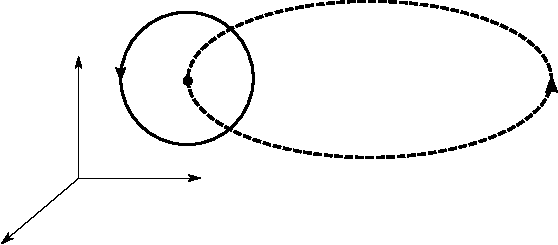
\includegraphics[width=\linewidth]{./centre_vortex.pdf}
\caption{\label{fig:CentreVortex} A single centre vortex (dashed line) intersecting a Wilson loop (solid line) in 3 dimensions. The Wilson loop will acquire a centre phase corresponding to the phase of the vortex.}
\end{figure}
%

Follwing the argument presented in Ref.~\cite{Makeenko:2009dw}, consider a Wilson loop calculated around a rectangle in the $x-t$ plane with dimensions $R\times T$. As the Wilson loop is gauge invariant, we are free to select a convenient gauge in which to perform the calculation. To this end, we choose the fields to be in axial gauge, such that $A_0(x)=0\implies U_0(x) = 1\,\forall\,x$. So the Wilson loop becomes
%
\begin{equation}
W(R\times T) = \Tr \left(U_1(0)\,U_1^\dagger(T)\right)\, .
\end{equation}
%
We can insert a complete set of energy eigenstates, $\sum_n |\,n\rangle\,\langle n \,|=1$ to obtain
%
\begin{align*}
W(R\times T) &= \Tr \left( \sum_n \langle U_1(0)\, |\, n\rangle\,\langle n\, |\, e^{-E_n(R)\, T}\, | \, U_1(0) \rangle\right)\\
&=  \sum_n \Tr \left( \big|\langle U_1(0)\, |\, n\rangle\big|^2 \right)\,e^{-E_n(R)\,T} 
\end{align*}
%
As $T\rightarrow \infty$, the only surviving contribution will be the lowest energy, $E_0(R)$. This means that
%
\begin{equation}
\lim_{T\rightarrow \infty} W(R\times T) \propto e^{-E_0(R)\, T}\, .
\label{eq:WilsonEnergy}
\end{equation}
\\

With Eq.~\ref{eq:WilsonEnergy} in mind, we return to the aforementioned $SU(3)$ confinement model. Consider a two-dimensional plane with area $L^2$, with $2N$ vortices piercing the plane. Assuming an even distribution of vortices, the total vortex density is $\rho = \frac{2N}{L^2}$. As there are two $SU(3)$ vortex types, corresponding to the two non-trivial phases $\exp\left(\frac{\pm 2\pi i}{3}\right)$, we assume that there is an equal distribution of vortex phases, i.e. there are $N$ vortices of each type. The probability of finding $n$ vortices of a given phase in some region of the plane $A\subseteq L^2$ is equal to the probability that exactly $n$ vortices are in $A$, multiplied by the probability that exactly $N-n$ vortices are outside of $A$, multiplied by the number of ways this situation can occur. Expressed mathematically, this is
%
\begin{equation}
P_N(n) = {N\choose n} \left(\frac{A}{L^2}\right)^n \left(1-\frac{A}{L^2}\right)^{N-n}\, .
\end{equation}
%
The expectation value of the Wilson loop around the perimeter of $A$ can be written as
%
\begin{equation}
\langle W(\partial A)\rangle = \sum_{m,n = 0}^N \left(\exp\left(\frac{2\pi i}{3}\right)\right)^n P_N(n)\, \left(\exp\left(\frac{2\pi i}{3}\right)\right)^m P_N(m)\, .
\end{equation}
%
If we assume the vortex phases are uncorrelated, then we can make use of the following property of uncorrelated random variables $X$ and $Y$
%
\begin{equation}
E[XY] = E[X]E[Y]\, ,
\end{equation}
%
to write
%
\begin{equation}
\langle W(\partial A)\rangle = \sum_{n=0}^N \left(\exp\left(\frac{2\pi i}{3}\right)\right)^n P_N(n)\,\sum_{m=0}^N \left(\exp\left(\frac{2\pi i}{3}\right)\right)^m P_N(m)\, .
\label{eq:WilsonExpectation}
\end{equation}
%
We consider just the first sum in Eq.~\ref{eq:WilsonExpectation} and calculate
%
\begin{align*}
\sum_{n=0}^N \left(\exp\left(\frac{2\pi i}{3}\right)\right)^n P_N(n) & = \left(1-\frac{A}{L^2}\right)^{N}\sum_{n=0}^{N} {N\choose n} \left(\exp\left(\frac{2\pi i}{3}\right)\,\frac{A}{L^2}\left(1-\frac{A}{L^2}\right)^{-1}\right)^n\\
&=\left(1+\left(\exp\left(\frac{2\pi i}{3}\right) - 1\right)\frac{A}{L^2}\right)^N\, ,
\end{align*}
%
where we have made use of the binomial series to evaluate the sum. Hence the total expectation value is
%
\begin{align}
\langle W(\partial A)\rangle &=\left(1+\left(\exp\left(\frac{2\pi i}{3}\right) - 1\right)\frac{A}{L^2}\right)^N\, \left(1+\left(\exp\left(\frac{-2\pi i}{3}\right) - 1\right)\frac{A}{L^2}\right)^N\nonumber\\
&=\left(1 -3\frac{A}{L^2} + 3\left(\frac{A}{L^2}\right)^2\right)^N\nonumber\\
&= \left(\left(\frac{A}{L^2}\right)^3+\left(1-\frac{A}{L^2}\right)^3\right)^N\, .\label{eq:WilsonExpectationSimple}
\end{align}
%
Rewriting Eq.~\ref{eq:WilsonExpectationSimple} in terms of the vortex density $\rho$, we have
%
\begin{equation}
\langle W(\partial A)\rangle = \left(\left(\frac{A\rho}{2N}\right)^3+\left(1-\frac{A\rho}{2N}\right)^3\right)^N\, .
\end{equation}
%
Now we take the limit as $N,L^2\rightarrow\infty$, keeping $\rho$ constant. Taking the limit, we find
%
\begin{equation}
\langle W(\partial A)\rangle = \exp\left(-\frac{3}{2}\rho A\right)
\label{eq:WilsonAreaLaw}
\end{equation}
%
Letting $A=R\times T$ as in Eq.~\ref{eq:WilsonEnergy}, we see that $E_0(R) = -\frac{3}{2}\rho R$, so the static quark potential rises linearly with distance between them, exactly as it should in a confining theory. Eq.~\ref{eq:WilsonAreaLaw} demonstrates an {\it area law} behaviour of the Wilson loop; this is often taken as a requirement for confinement~\cite{DelDebbio:1998luz,Dosch:1988ha}.\\

%
\begin{figure}[h]
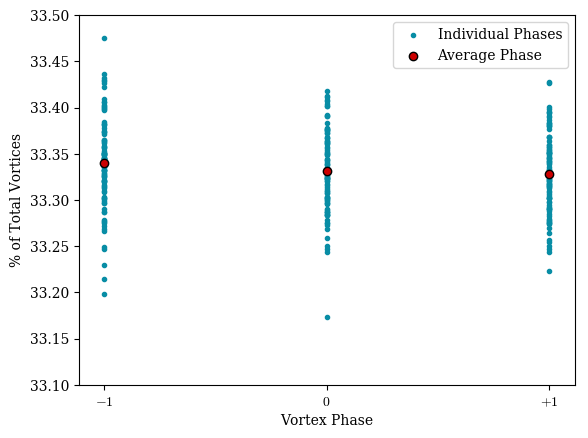
\includegraphics{./VortexDistribution.png}
\caption{\label{fig:VortexDistribution}A plot of the vortex phase distribution of 100 Monte-Carlo generated configurations, as a percentage of the total number of vortices. The method by which vortices are identified will be detailed in Sec.~\ref{sec:LocatingVortices}.}
\end{figure}
%
It is important to highlight the assumptions and simplifications made in the above argument. Most easily addressed is the assumption that there is an equal number of $+1$ and $-1$ vortices. By identifying vortices in Monte-Carlo generated configurations and plotting the distribution of phases in Fig.~\ref{fig:VortexDistribution}, we see that there is little deviation from an even distribution, especially in the ensemble average. This is an expected result, as we shall see later that vortices are required to form closed loops in 3D to conserve the vortex flux, so a vortex line should pierce a 2D surface once in each direction, corresponding to the two non-trivial phases.\\

The assumption that the vortex density is constant is, however, less well motivated. So far we have treated vortices as infinitesimally thin sheets in 4D, which is not physically motivated. An infinitely thin vortex introduces a singularity in the action, as the vortex flux must be constrained to an infinitely thin cross-section. Rather, physical vortices are `thick'; they have a finite cross-section in the direction perpendicular to the vortex sheet. If the vortex is contained entirely within the area $A$ it contributes the centre phase as described above. However, as $A$ approaches the size of the vortex cross section, one must account for vortices that are only partially inside $A$, and thus not necessarily contributing a pure centre phase. Although this consideration spoils the elegance of the above confinement mechanism for small Wilson loops, it does potentially save the model from a previously noted pitfall related to the Casimir scaling of the Wilson loop expectation value~\cite{Greensite:1982be}, as will be described in more detail in Sec.~\ref{}. Finally, it is worth noting that this issue is only relevant to Wilson loops of similar size to the vortex cross-section. As the Wilson loop increases in size, the majority of the vortices will be contained entirely within the loop, with a diminishing number of thick vortices overlapping the perimeter of the loop, as shown in Fig.~\ref{fig:VortexSizes}.\\
%
\begin{figure}[htb!]
\centering
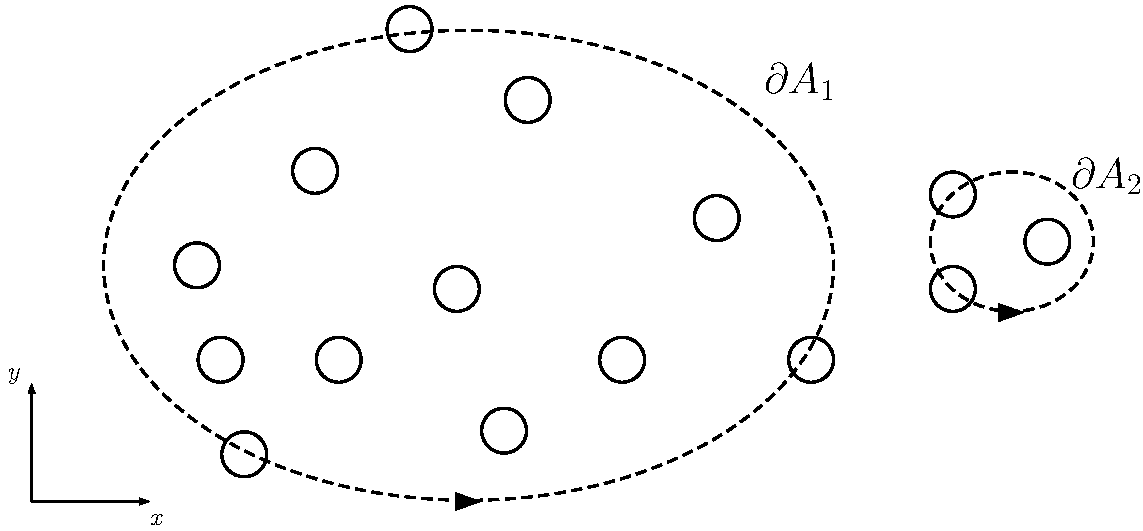
\includegraphics[width=\linewidth]{./LargeVortex.pdf}
\caption{\label{fig:VortexSizes}An example of two Wilson loops (dashed lines) lying in a plane, pierced by vortices of finite cross-section (solid lines). \textbf{Left:} The majority of vortices contributing to the phase are fully contained within the large loop, with only a few overlapping at the perimeter. \textbf{Right:} For a small loop, the contribution from overlapping vortices is significant as there are few vortices fully inside the loop.}
\end{figure}

The final assumption is that the vortex locations are random and uncorrelated from one another. This is perhaps the most significant assumption made in the above picture, as can be seen from the following calculation~\cite{Engelhardt:1999fd}. As vortices must form closed lines in 3D, let us suppose that instead of being randomly distributed, the vortices come in pairs separated by a maximum distance $d$. This corresponds to requiring that vortex lines form a closed loop of some maximum diameter $d$. If this vortex line pierces the Wilson loop in both directions, then the product of the phases, $\exp\left(\frac{2\pi i}{3}\right)\times \exp\left(\frac{-2\pi i}{3}\right) = 1$, results in no contribution to the Wilson loop. Hence, the only vortices capable of contributing a non-trivial phase to the Wilson loop are those contained within a strip of width $d$ about the perimeter of the loop. Note that not every vortex within this strip will contribute a non-trivial phase, as for example the vortex may be smaller than $d$ or oriented such that the vortex flows in direction of $\partial A$ and thus still pierces twice. We will take the most generous case, however, and assume that every vortex piercing this strip contributes a non-trivial phase. To first order, the area of relevance to to the expectation value of the Wilson loop is now $A_\text{strip}=\partial A\, d$. The probability to find $N$ vortices lying within this strip is 
%
\begin{equation}
P_N(n) = {N\choose n} \left(\frac{\partial A d}{L^2}\right)^n \left(1-\frac{\partial A d}{L^2}\right)^{N-n}\, .
\end{equation}
%
By following the same steps used to arrive at Eq.~\ref{eq:WilsonAreaLaw}, we find
%
\begin{equation}
\langle W(\partial A)\rangle = e^{-\frac{3}{2}\rho\, d\, \partial A}\, .
\end{equation}
%
So we see that instead of an area law, we now have a perimeter law for the Wilson loop, dependent on the upper bound for the vortex size. This implies that if there is some upper limit on the size of a vortex, we can no longer expect to see confining behaviour. We deduce therefore that to obtain a confining theory, it is necessary to allow the vortex size to be potentially infinite. In the language of the vortex model, this is called \textit{vortex percolation}. Conversely, the presence of an upper bound on the vortex size would imply a deconfined phase. This suggests that the size of vortices can be used as an \textit{order parameter} for confinement~\cite{Langfeld:1998cz}, with two distinct phases:
\begin{enumerate}
\item Vortex percolation $\implies$ confinement.
\item Loss of vortex percolation $\implies$ deconfinement.
\end{enumerate}
\subsection{Current Evidence for Centre Vortices}
\subsubsection{String Tension}

\subsubsection{Hadron Spectrum}

\subsubsection{Mass Function}

\subsubsection{Gluon Propagator}

\subsubsection{Casimir Scaling}


\section{Locating Centre Vortices}\label{sec:LocatingVortices}
\subsection{Maximal Centre Gauge}\label{sec:MCG}
\subsection{Centre Projection}
\section{Further Topological Quantities}
\subsection{Instantons}
\subsection{Topological Charge}

%A frequently seen mistake is to use `\textbackslash begin\{center\}' \dots `\textbackslash end\{center\}' inside a figure or table environment. This center environment can cause additional vertical space. If you want to avoid that just use `\textbackslash centering'
%
%
%\begin{table}
%\caption{A badly formatted table}
%\centering
%\label{table:bad_table}
%\begin{tabular}{|l|c|c|c|c|}
%\hline 
%& \multicolumn{2}{c}{Species I} & \multicolumn{2}{c|}{Species II} \\ 
%\hline
%Dental measurement  & mean & SD  & mean & SD  \\ \hline 
%\hline
%I1MD & 6.23 & 0.91 & 5.2  & 0.7  \\
%\hline 
%I1LL & 7.48 & 0.56 & 8.7  & 0.71 \\
%\hline 
%I2MD & 3.99 & 0.63 & 4.22 & 0.54 \\
%\hline 
%I2LL & 6.81 & 0.02 & 6.66 & 0.01 \\
%\hline 
%CMD & 13.47 & 0.09 & 10.55 & 0.05 \\
%\hline 
%CBL & 11.88 & 0.05 & 13.11 & 0.04\\ 
%\hline 
%\end{tabular}
%\end{table}
%
%\begin{table}
%\caption{A nice looking table}
%\centering
%\label{table:nice_table}
%\begin{tabular}{l c c c c}
%\hline 
%\multirow{2}{*}{Dental measurement} & \multicolumn{2}{c}{Species I} & \multicolumn{2}{c}{Species II} \\ 
%\cline{2-5}
%  & mean & SD  & mean & SD  \\ 
%\hline
%I1MD & 6.23 & 0.91 & 5.2  & 0.7  \\
%
%I1LL & 7.48 & 0.56 & 8.7  & 0.71 \\
%
%I2MD & 3.99 & 0.63 & 4.22 & 0.54 \\
%
%I2LL & 6.81 & 0.02 & 6.66 & 0.01 \\
%
%CMD & 13.47 & 0.09 & 10.55 & 0.05 \\
%
%CBL & 11.88 & 0.05 & 13.11 & 0.04\\ 
%\hline 
%\end{tabular}
%\end{table}
%
%
%\begin{table}
%\caption{Even better looking table using booktabs}
%\centering
%\label{table:good_table}
%\begin{tabular}{l c c c c}
%\toprule
%\multirow{2}{*}{Dental measurement} & \multicolumn{2}{c}{Species I} & \multicolumn{2}{c}{Species II} \\ 
%\cmidrule{2-5}
%  & mean & SD  & mean & SD  \\ 
%\midrule
%I1MD & 6.23 & 0.91 & 5.2  & 0.7  \\
%
%I1LL & 7.48 & 0.56 & 8.7  & 0.71 \\
%
%I2MD & 3.99 & 0.63 & 4.22 & 0.54 \\
%
%I2LL & 6.81 & 0.02 & 6.66 & 0.01 \\
%
%CMD & 13.47 & 0.09 & 10.55 & 0.05 \\
%
%CBL & 11.88 & 0.05 & 13.11 & 0.04\\ 
%\bottomrule
%\end{tabular}
%\end{table}
